\documentclass[a4paper,12pt]{article}
\usepackage{graphicx}       %LaTeX package to import graphics

\usepackage[T1]{fontenc}
\usepackage[italian]{babel}

\usepackage{subcaption}

\usepackage{hyphenat}
\usepackage{array}
\usepackage{booktabs}       % Per linee orizzontali migliori
\usepackage{caption}        % Per personalizzare le didascalie<
\usepackage{multirow}       % Per combinare celle nelle colonne
\usepackage{float}
\usepackage{hyperref}

\usepackage{bm} 

\usepackage{amsmath}        % Per migliorare l'aspetto delle formule

\usepackage{todonotes}      % mettere le note dentro il documento

\usepackage{siunitx}        % Per formattare le unità di misura
\usepackage{gensymb}        % Simboli come °
\usepackage{xfrac}          % per fare le frazioni inclinate

\usepackage{pdfpages}

\usepackage{import}
\usepackage{frontespizio}

\usepackage{placeins}       %per non far andare le immagini al di fuori delle sezioni utilizzare il comando: \FloatBarrier non far superare le immagini quel punto

\usepackage{adjustbox}      % per dimensionare le immagini in modo automatico


\begin{document}

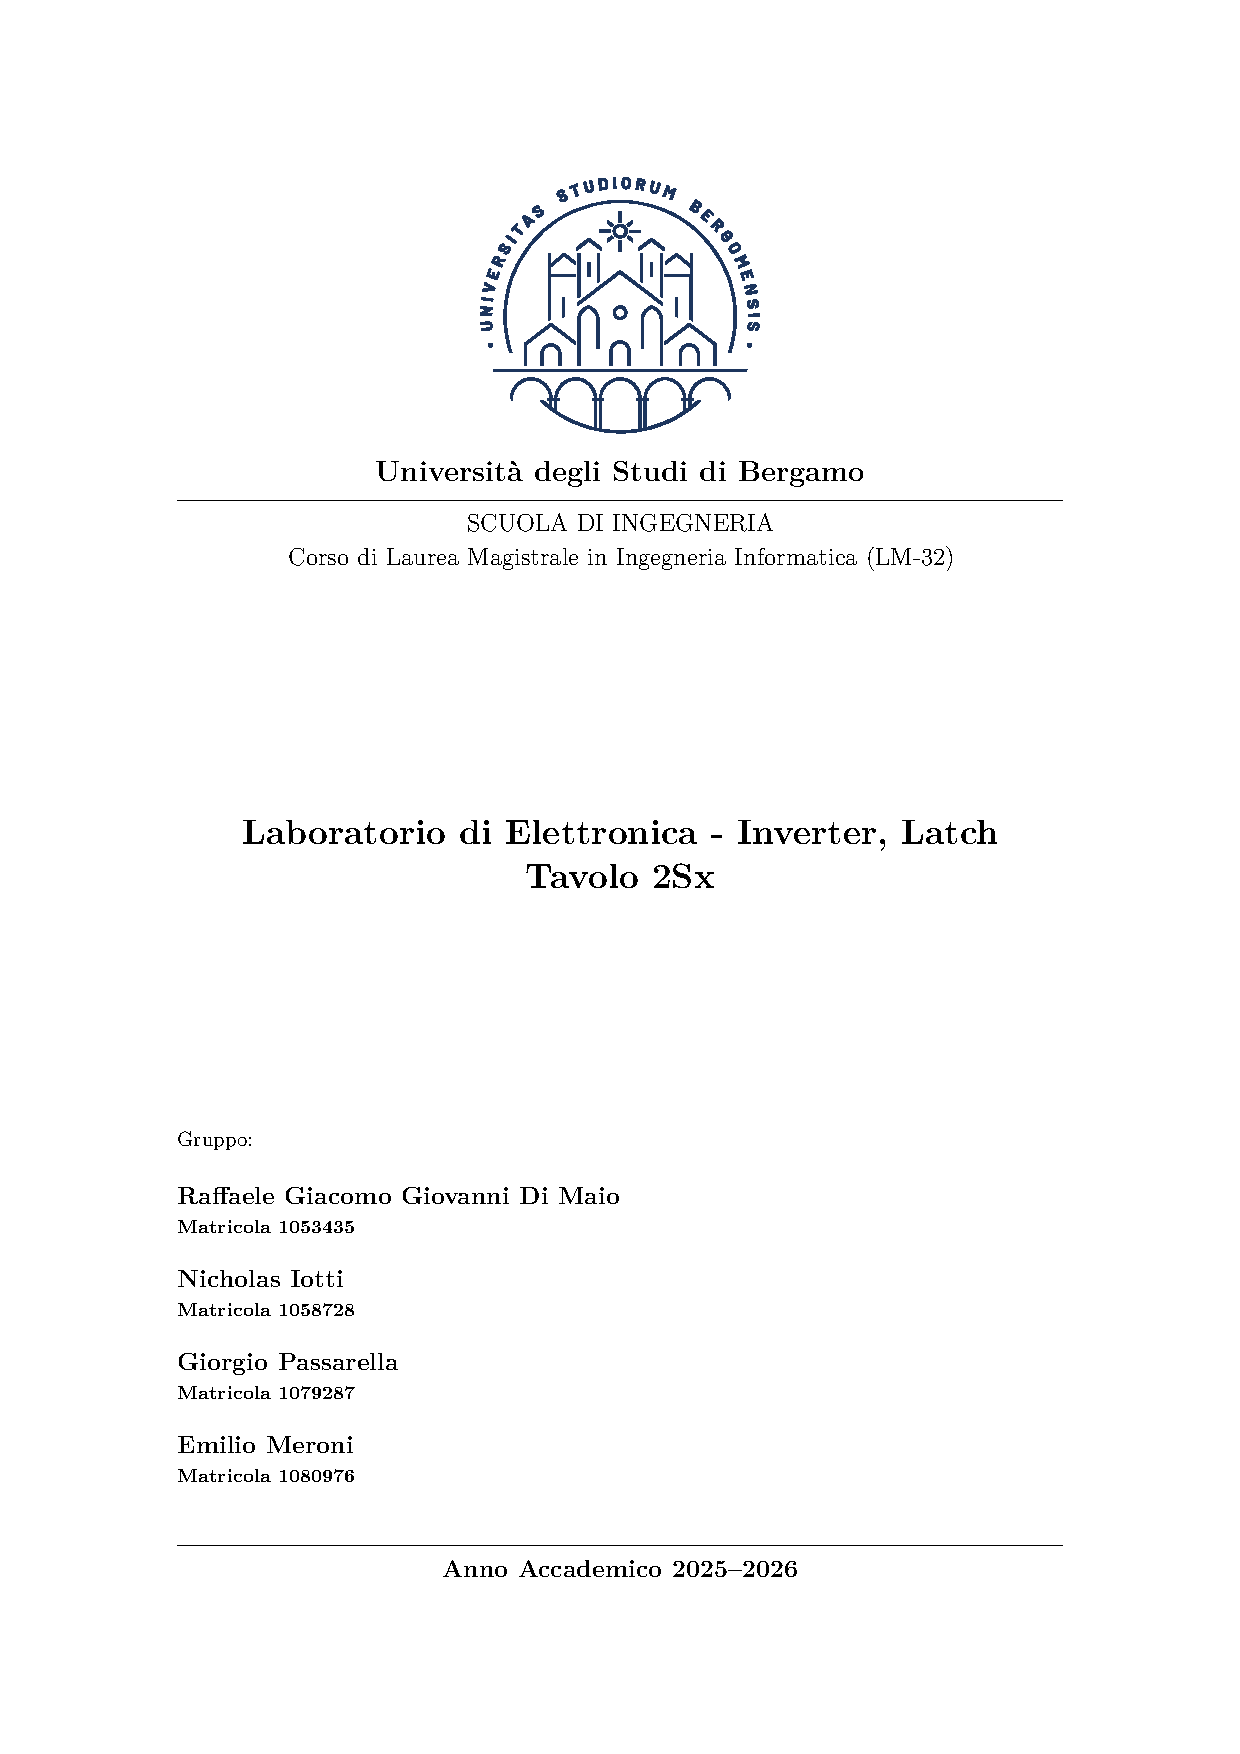
\includepdf{./frontespizio/frontespizio.pdf}

\section*{Inverter CMOS}
\begin{figure}[H]
	\centering
	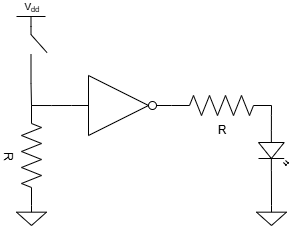
\includegraphics[width=0.5\linewidth]{immagini/inverter/circuitoLogico1Led.png}
	\caption{Schematico inverter.}
	\label{fig:inverterStatica}
\end{figure}
Per la realizzazione del circuito mostrato in \autoref{fig:inverterStatica} è stato utilizzato il circuito integrato \textbf{CB4069}, tale dispositivo è dotato di 14 pin: il pin 14 è collegato alla tensione positiva di alimentazione, mentre il pin 7 è collegato a massa, tutti gli altri pin rappresentano gli ingressi e le uscite dei sei inverter integrati (da $A$ e $\overline{A}$ fino a $F$ e $\overline{F}$).
È stata impostata una \textbf{V\textsubscript{DD}} di \SI{5}{\volt} con l’obiettivo di verificare la \textbf{caratteristica statica} dell’inverter. 
Per farlo, si forza uno stato logico 0 o 1 utilizzando una resistenza in serie a un interruttore collegato all’ingresso dell’inverter. 
In uscita è stata posta una resistenza con in serie un diodo LED, in modo che con uscita logica 1 il LED risulti acceso e con uscita logica 0 risulti spento come mostrato in \autoref{fig:statica}.
Successivamente andando a modificare il circuito come in \autoref{fig:inverterDinamica}, è stato possibile verificare la \textbf{caratteristica dinamica} collegando l’ingresso del circuito a un generatore di forme d’onda che fornisce un segnale ad onda quadra con un’ampiezza di \SI{5}{\volt\text{-picco-picco}} e un offset di \SI{2.5}{\volt}, simulando la commutazione di un bit tra 0 e 1, per osservare la negazione in uscita. 
Infine, sono stati calcolati il \textbf{tempo di salita}, il \textbf{tempo di discesa} e il \textbf{ritardo di propagazione} dell’inverter. 
In \autoref{fig:ritardo_propagazione} è riportata la misura del ritardo di propagazione, pari a circa \SI{23.6}{\nano\second}. 
Le \autoref{fig:salita} e \autoref{fig:discesa} mostrano rispettivamente i fronti di salita e discesa del segnale in uscita, con tempi pari a circa \SI{30}{\nano\second} e \SI{20}{\nano\second}. 

\begin{figure}[H]
    \centering
    \begin{subfigure}[b]{0.45\textwidth}
        \centering
        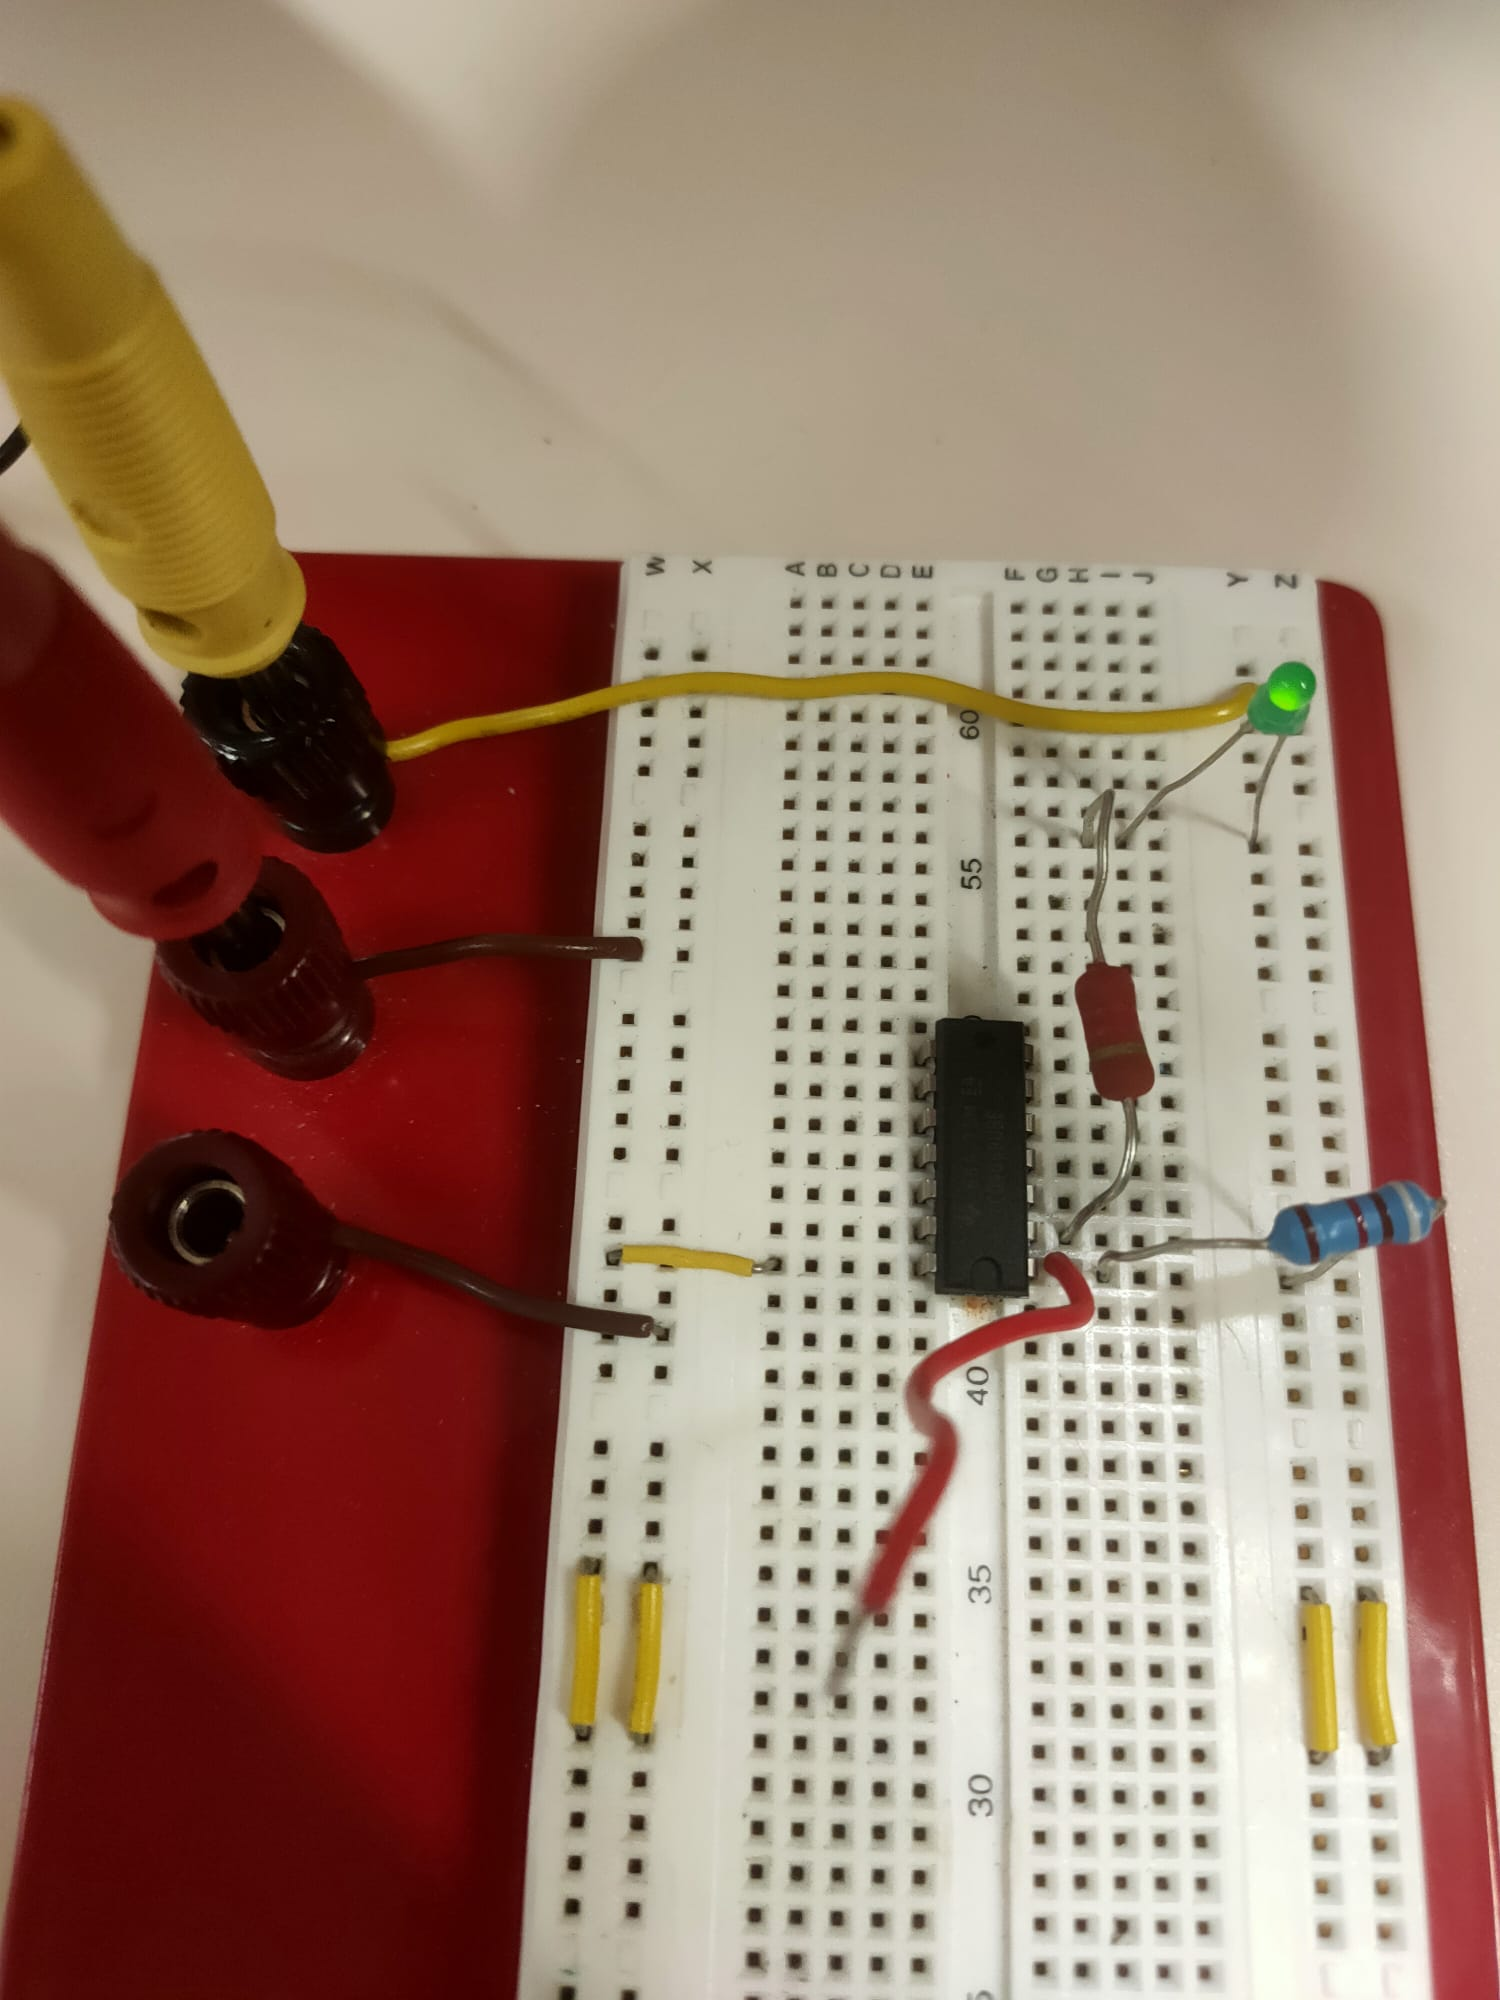
\includegraphics[width=\textwidth]{immagini/inverter/on.png}
        \caption{Uscita logica 1 – LED acceso}
        \label{fig:led_on}
    \end{subfigure}
    \hfill
    \begin{subfigure}[b]{0.45\textwidth}
        \centering
        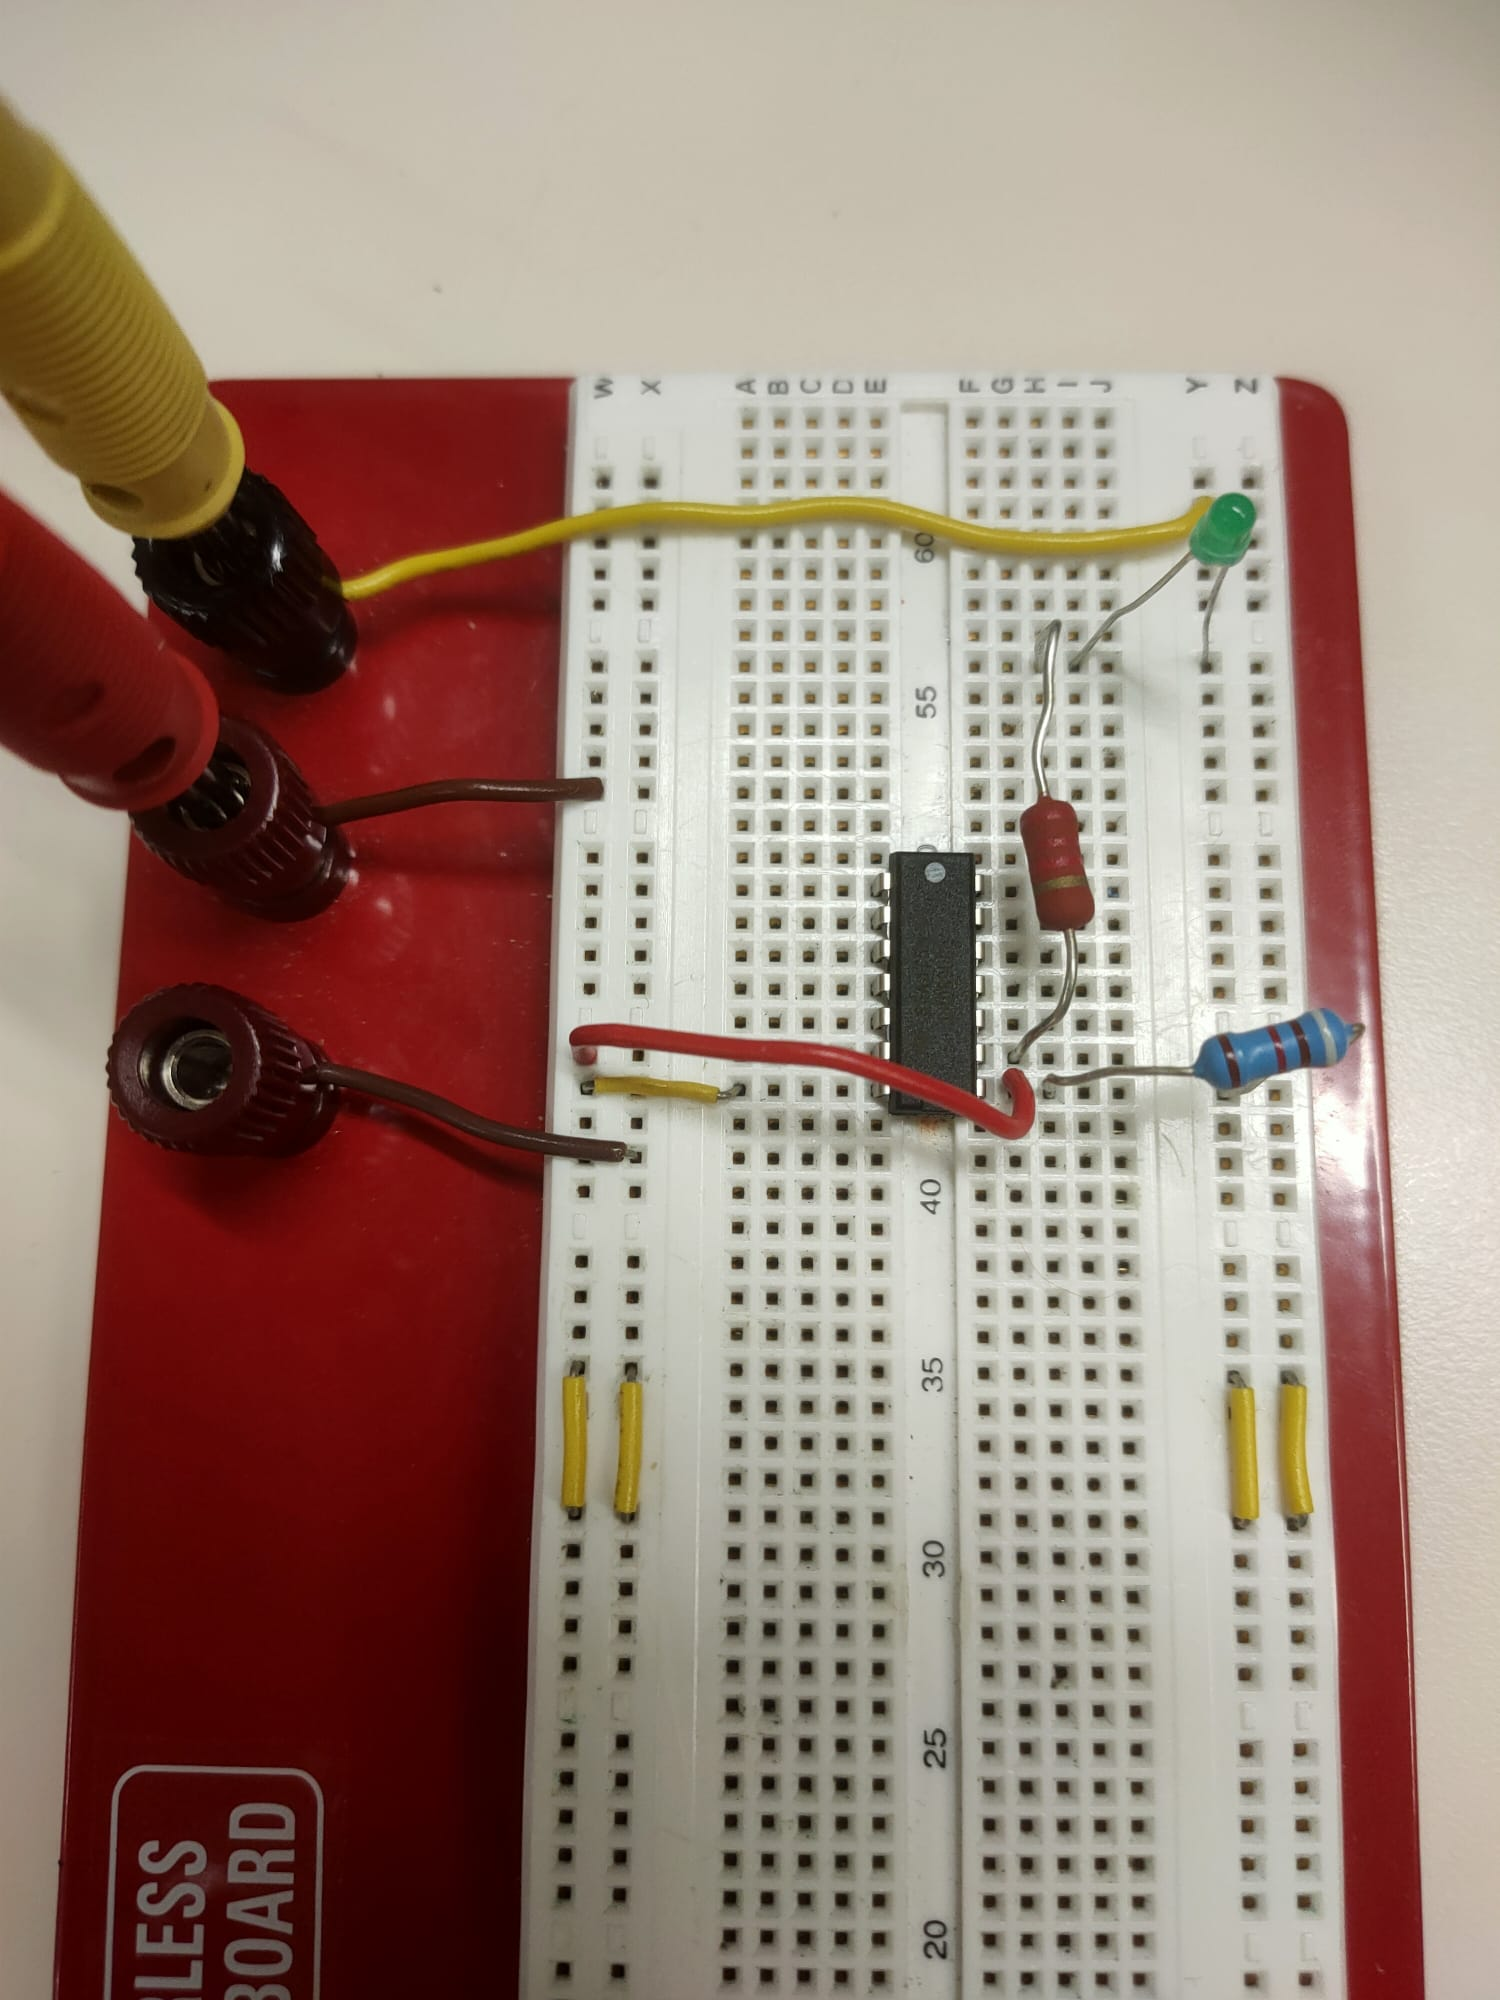
\includegraphics[width=\textwidth]{immagini/inverter/off.png}
        \caption{Uscita logica 0 – LED spento}
        \label{fig:led_off}
    \end{subfigure}
    \caption{Verifica della caratteristica statica dell'inverter tramite LED}
    \label{fig:statica}
\end{figure}

\begin{figure}[H]
    \centering
    
    \begin{subfigure}[b]{0.45\textwidth}
        \centering
        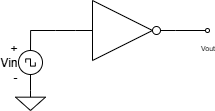
\includegraphics[width=\linewidth]{immagini/inverter/circuitoLogico1NoLed.png}
        \caption{Schematico dell'inverter per la verifica della caratteristica dinamica.}
        \label{fig:inverterDinamica}
    \end{subfigure}
    \hfill
    \begin{subfigure}[b]{0.45\textwidth}
        \centering
        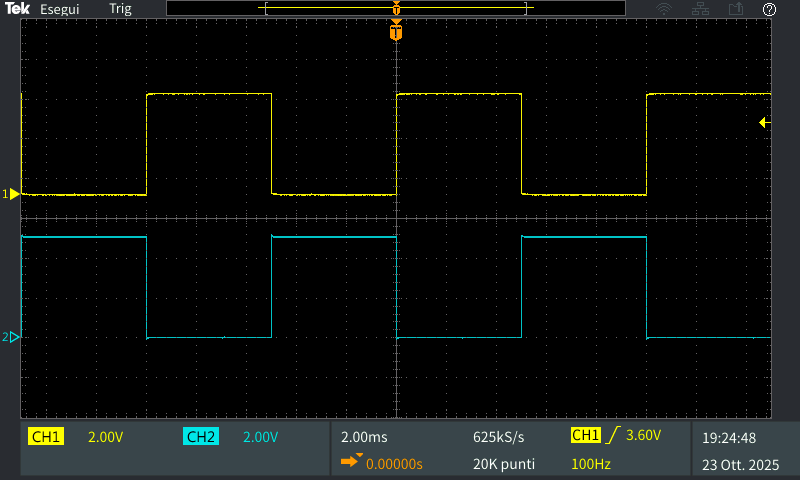
\includegraphics[width=\linewidth]{immagini/inverter/TEK00099.PNG}
        \caption{Caratteristica dinamica dell'inverter.}
        \label{grafico}
    \end{subfigure}
    \caption{Verifica della caratteristica dinamica dell'inverter: a sinistra lo schema del circuito, a destra la risposta osservata all'oscilloscopio.}
    \label{fig:inverterDinamica}
\end{figure}

\begin{figure}[H]
    \centering
    \begin{subfigure}[b]{0.48\textwidth}
        \centering
        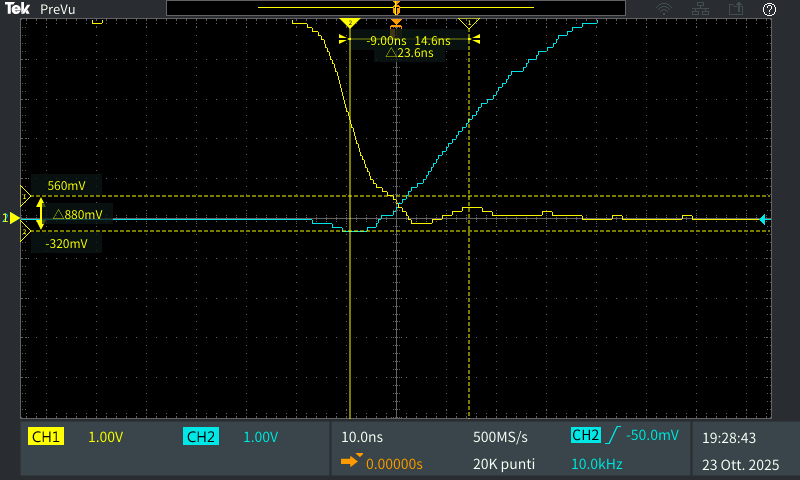
\includegraphics[width=\linewidth]{immagini/inverter/TEK00100.PNG}
        \caption{Ritardo di propagazione (\SI{23.6}{\nano\second}).}
        \label{fig:ritardo_propagazione}
    \end{subfigure}
    \hfill
    \begin{subfigure}[b]{0.48\textwidth}
        \centering
        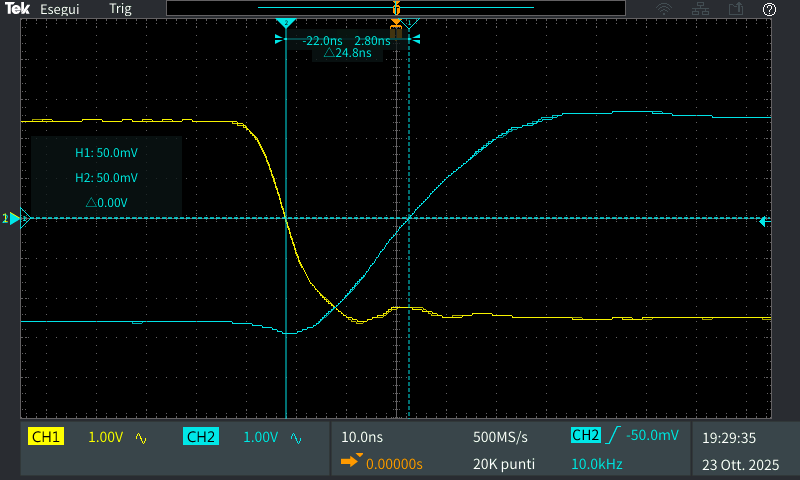
\includegraphics[width=\linewidth]{immagini/inverter/TEK00101.PNG}
        \caption{Transizioni complete.}
        \label{fig:transizioni_complete}
    \end{subfigure}
    \\[1em]
    \begin{subfigure}[b]{0.48\textwidth}
        \centering
        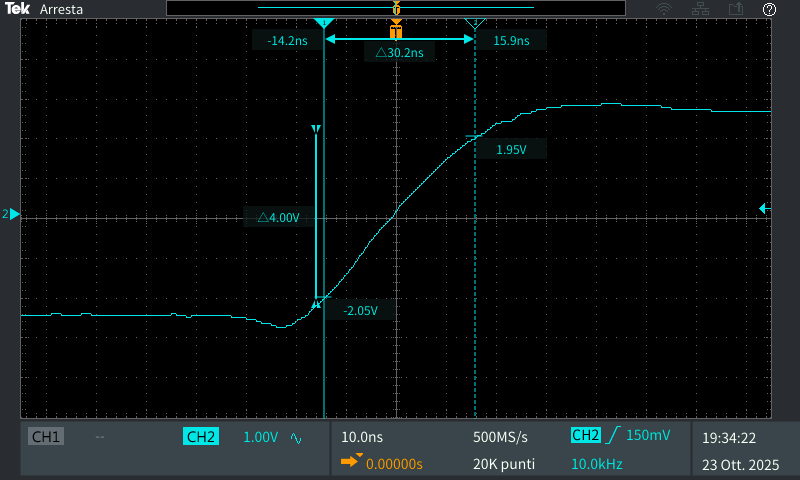
\includegraphics[width=\linewidth]{immagini/inverter/TEK00102.PNG}
        \caption{Tempo di salita (\SI{30}{\nano\second}).}
        \label{fig:salita}
    \end{subfigure}
    \hfill
    \begin{subfigure}[b]{0.48\textwidth}
        \centering
        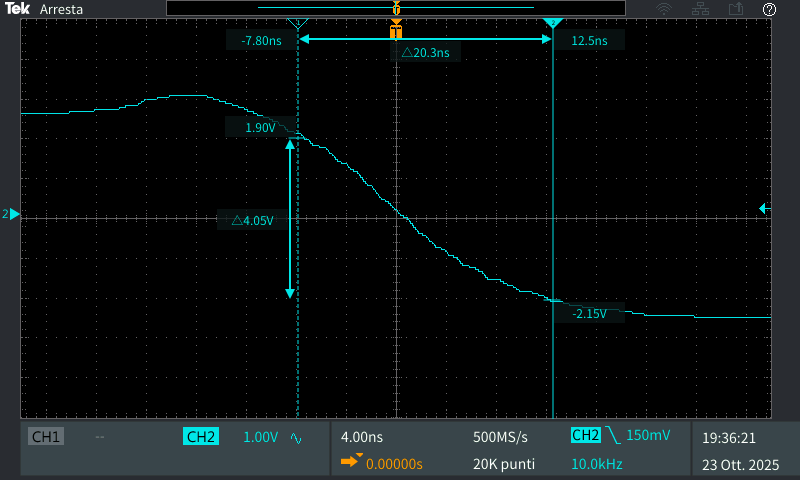
\includegraphics[width=\linewidth]{immagini/inverter/TEK00103.PNG}
        \caption{Tempo di discesa (\SI{20}{\nano\second}).}
        \label{fig:discesa}
    \end{subfigure}
    \caption{Misure sperimentali della caratteristica dinamica dell'inverter CMOS.}
    \label{fig:dinamica_misure}
\end{figure}

\section{Latch}

Il latch rappresenta una cella di memoria elementare, in grado di mantenere lo stato logico impostato anche dopo la rimozione del segnale di ingresso.  
Il suo principio di funzionamento si basa sull’impiego di due inverter collegati in cascata e retroazionati, come mostrato nello schema in \autoref{fig:latch_schema}.  
Quando viene applicato un livello logico 1 all’ingresso del primo inverter, la sua uscita assume valore logico 0, che a sua volta viene invertito dal secondo stadio, restituendo un livello logico 1.  
Questo valore viene quindi mantenuto grazie all’anello di retroazione, che stabilizza il circuito nello stato logico impostato.  
Un comportamento analogo si verifica quando viene applicato un livello logico 0: l’uscita del secondo inverter rimane a 0 fino a quando non interviene una nuova scrittura.
Per consentire la scrittura di uno stato logico, il circuito è stato dotato di due pulsanti: 
uno collegato alla tensione di alimentazione \textbf{V\textsubscript{DD}} per impostare un livello logico alto, e uno collegato a massa per impostare un livello logico basso. 
L’uscita è stata collegata a un LED per rendere visibile lo stato memorizzato: come mostrato in \autoref{fig:latch_onoff}, quando l’uscita è a livello logico 1 il LED risulta acceso, mentre con livello logico 0 rimane spento.
\begin{figure}[H]
    \centering
    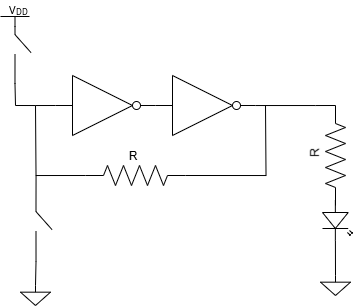
\includegraphics[width=0.6\linewidth]{immagini/latch/Latch.png}
    \caption{Schema circuitale del latch.}
    \label{fig:latch_schema}
\end{figure}

\begin{figure}[H]
    \centering
    \begin{subfigure}[b]{0.47\textwidth}
        \centering
        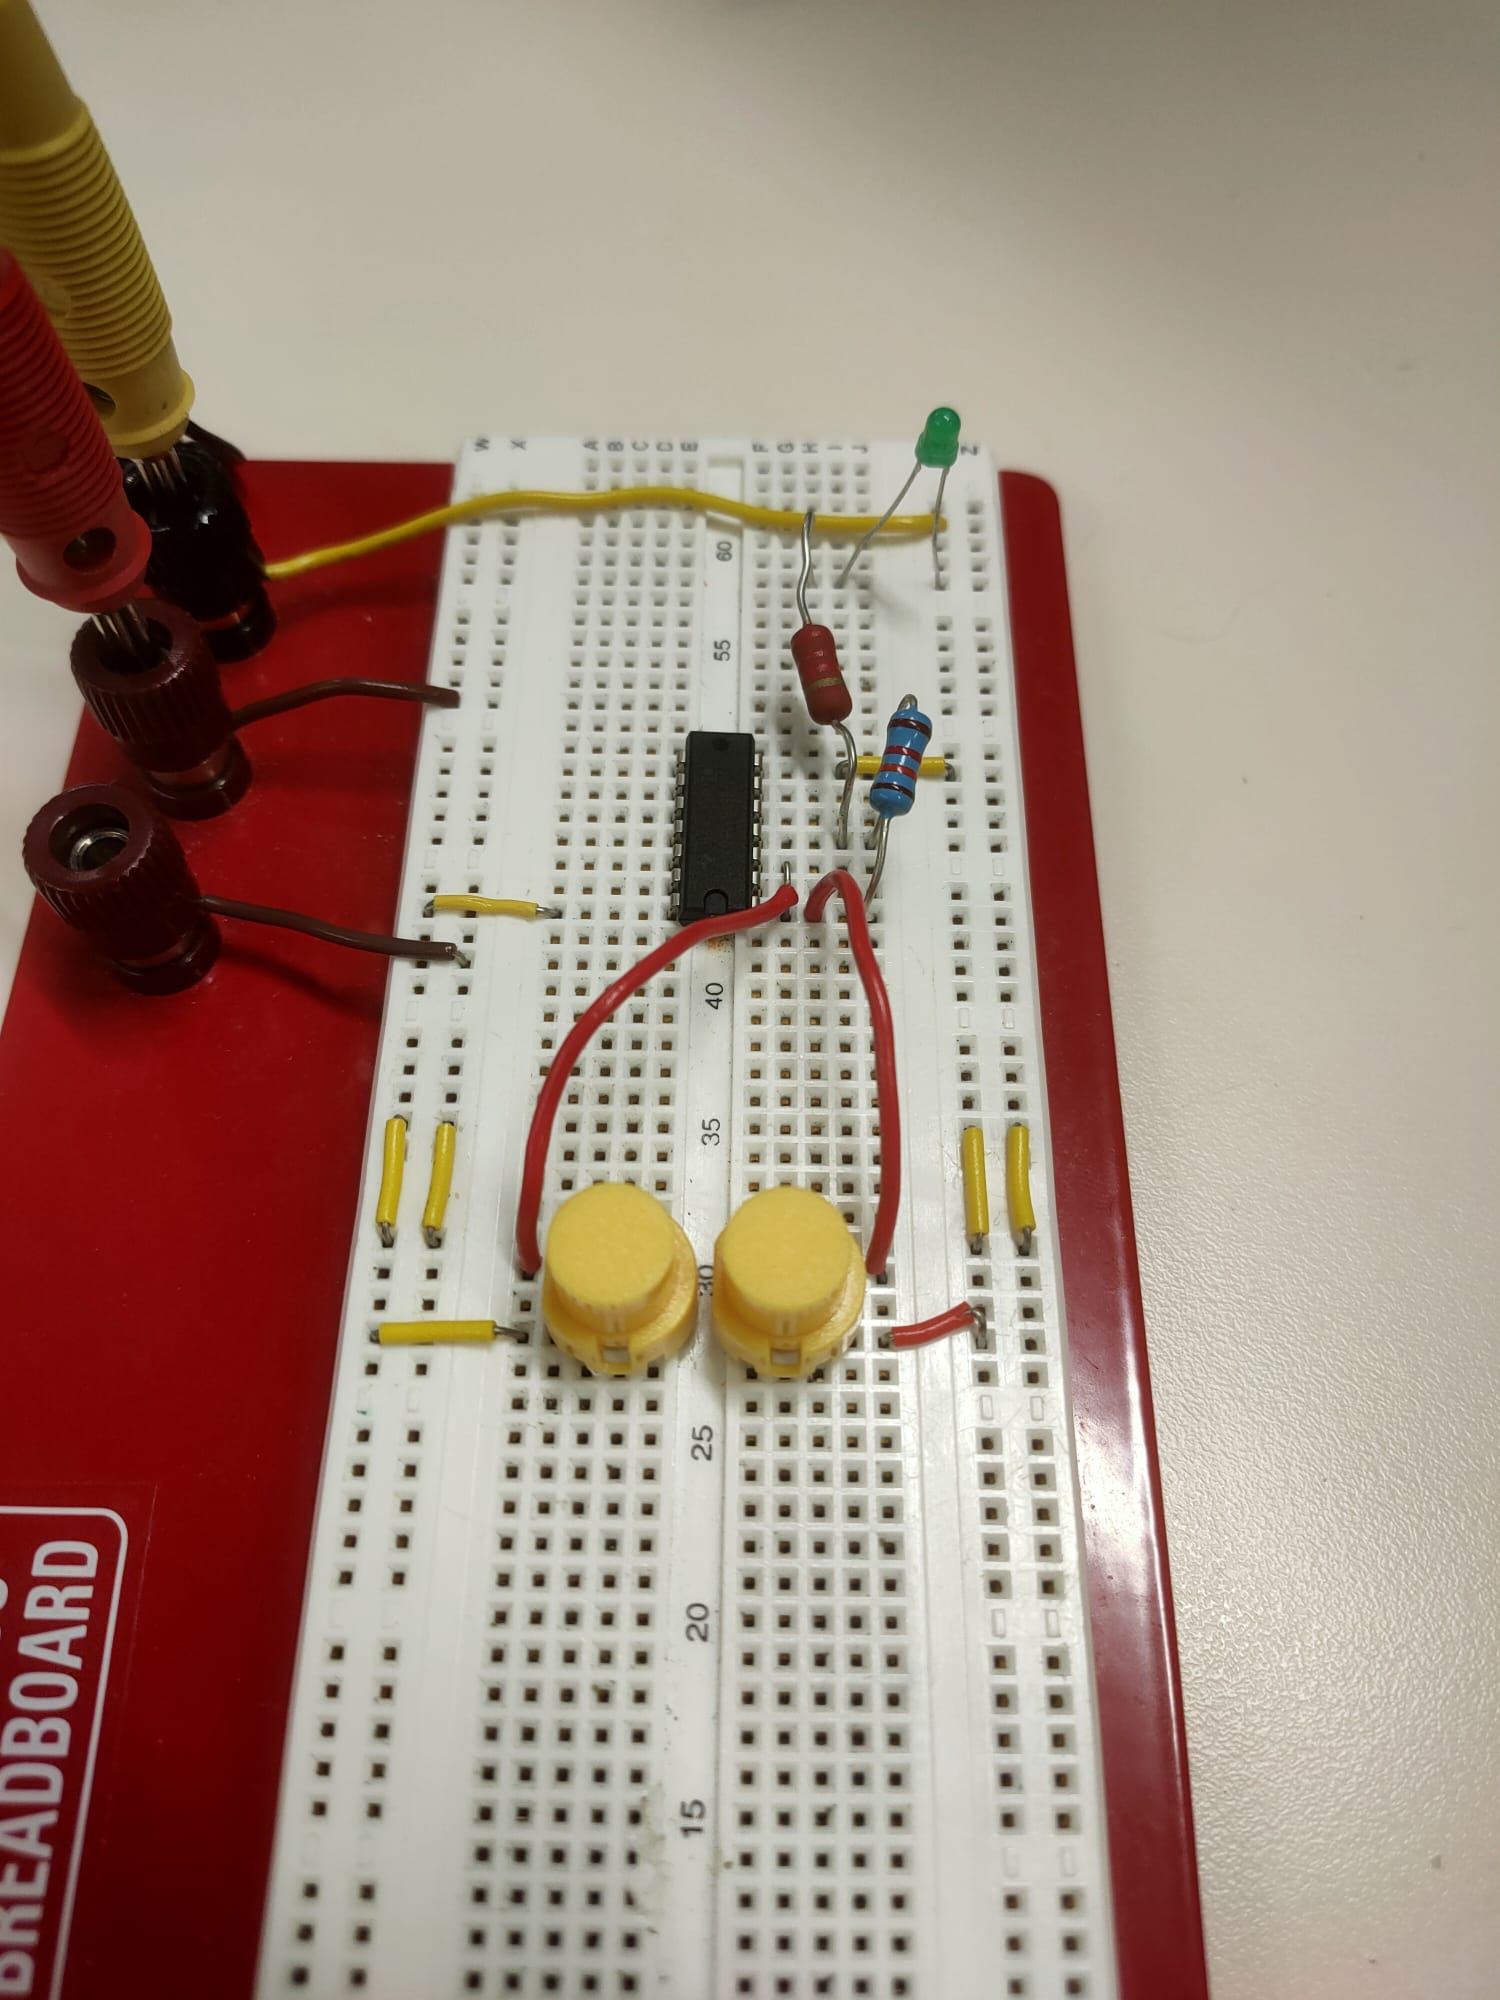
\includegraphics[width=\linewidth]{immagini/latch/off.png}
        \caption{Uscita logica 0, LED spento.}
    \end{subfigure}
    \hfill
    \begin{subfigure}[b]{0.47\textwidth}
        \centering
        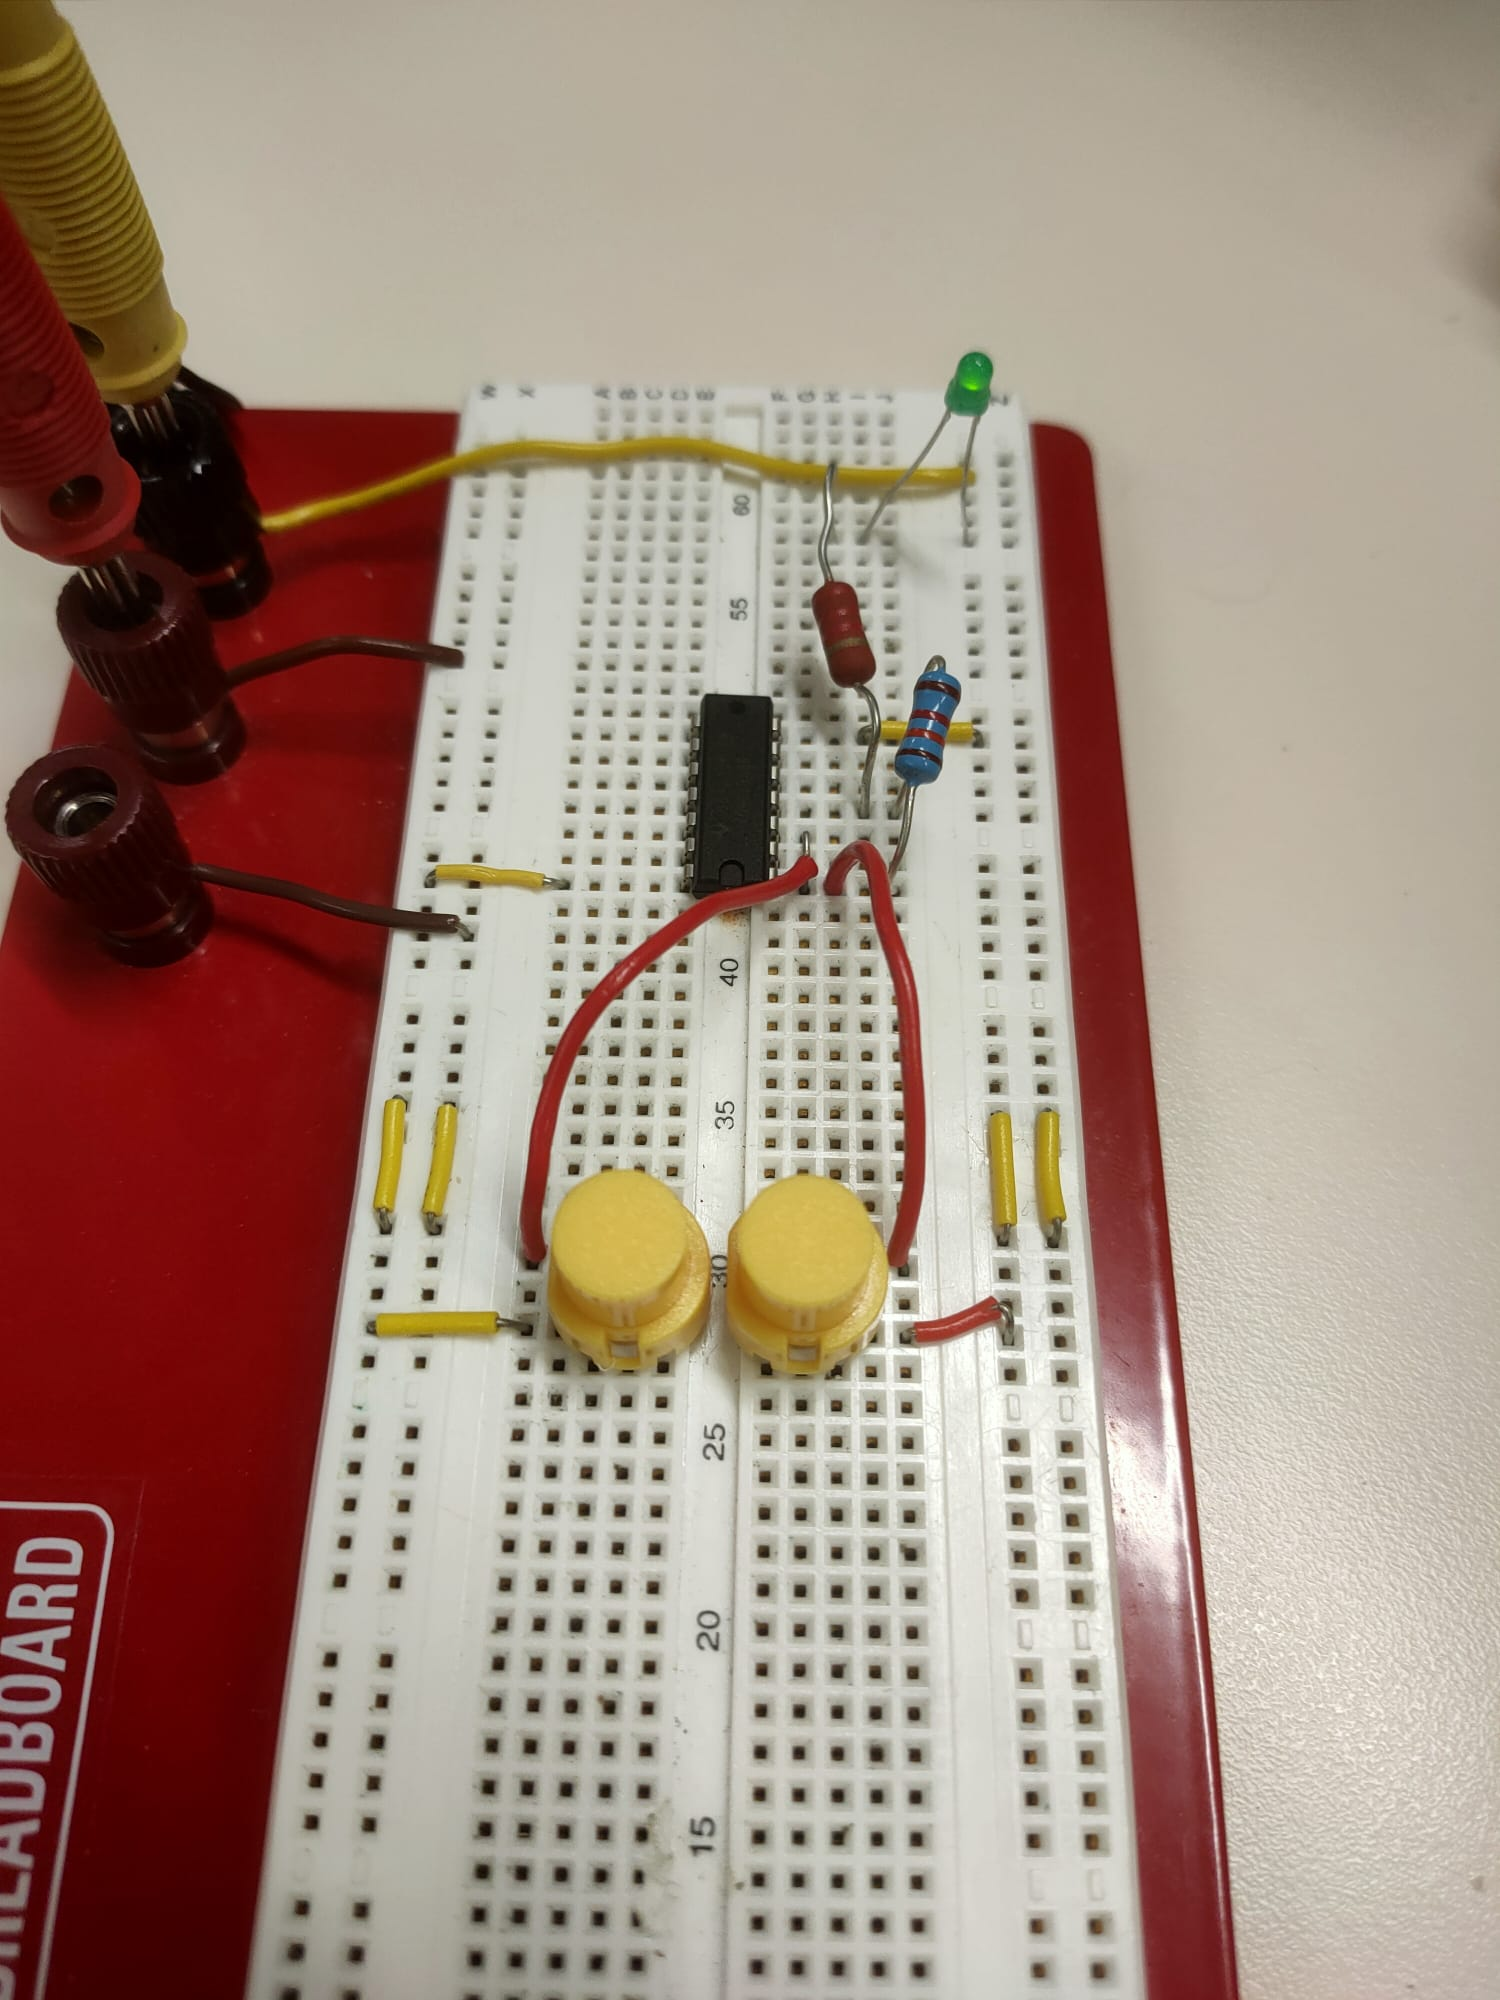
\includegraphics[width=\linewidth]{immagini/latch/on.png}
        \caption{Uscita logica 1, LED acceso.}
    \end{subfigure}
    \caption{Stati logici  dal latch.}
    \label{fig:latch_onoff}
\end{figure}



\end{document}

